\chapter{Практические задания}

\section{Задание 1. Составить диаграмму вычисления выражений}

На рисунках \ref{1_1}~--~\ref{1_6} представлены диаграммы вычисления выражений.

\begin{figure}[H]
	\centering
	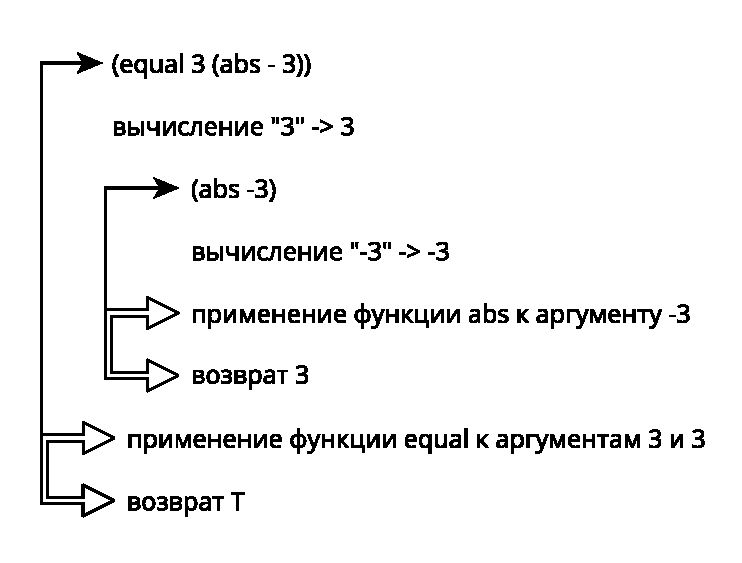
\includegraphics[width=0.5\linewidth]{1_1}
	\caption{Диаграмма вычисления выражения (equal 3 (abs - 3))}
	\label{1_1}
\end{figure}
\begin{figure}[H]
	\centering
	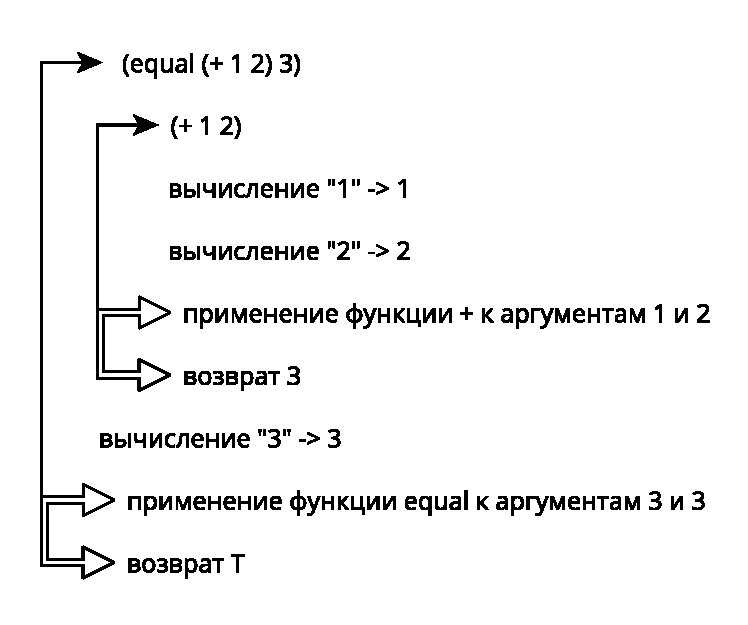
\includegraphics[width=0.5\linewidth]{1_2}
	\caption{Диаграмма вычисления выражения (equal (+ 1 2) 3)}
	\label{1_2}
\end{figure}
\begin{figure}[H]
	\centering
	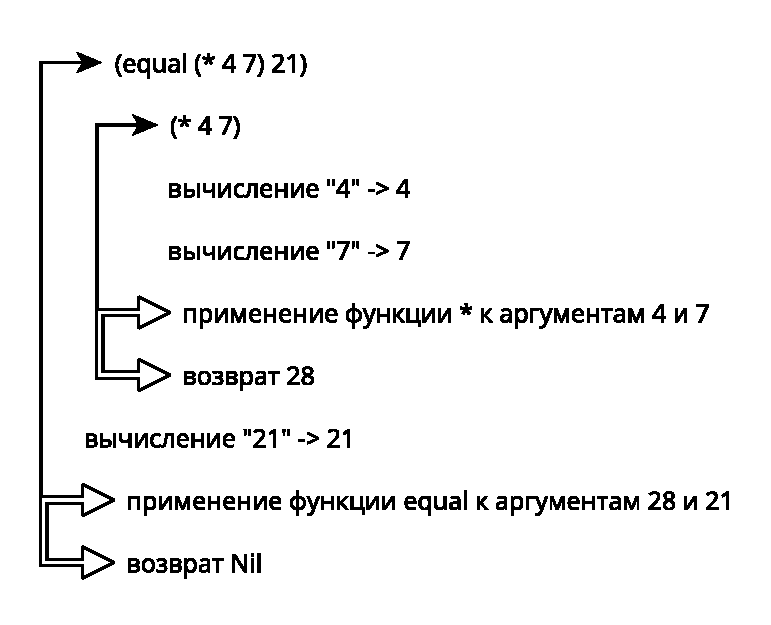
\includegraphics[width=0.5\linewidth]{1_3}
	\caption{Диаграмма вычисления выражения (equal (* 4 7) 21)}
	\label{1_3}
\end{figure}
\begin{figure}[H]
	\centering
	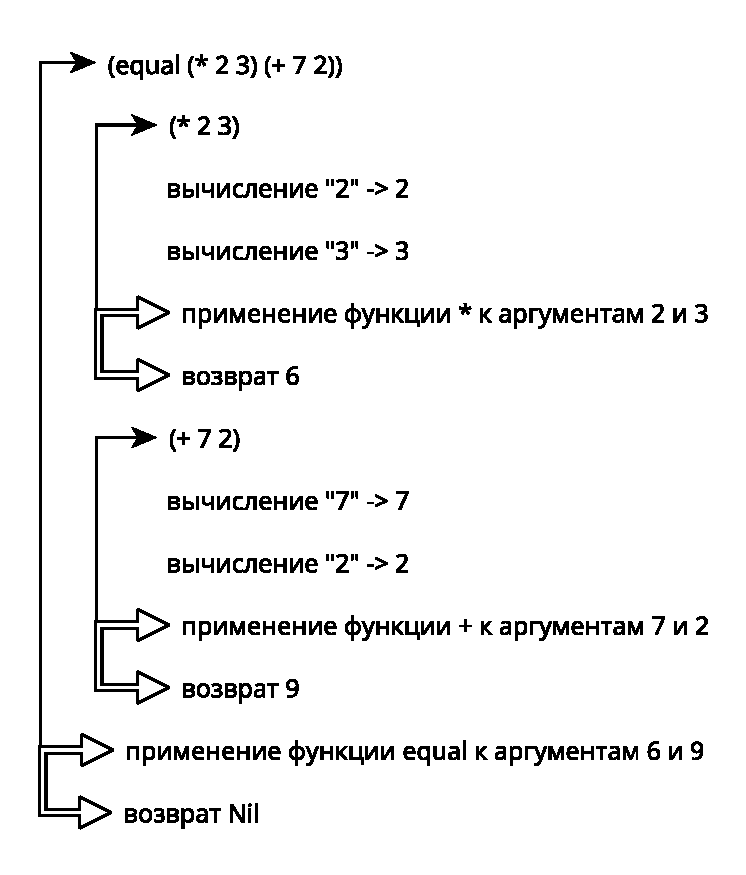
\includegraphics[width=0.5\linewidth]{1_4}
	\caption{Диаграмма вычисления выражения (equal (* 2 3) (+ 7 2))}
	\label{1_4}
\end{figure}
\begin{figure}[H]
	\centering
	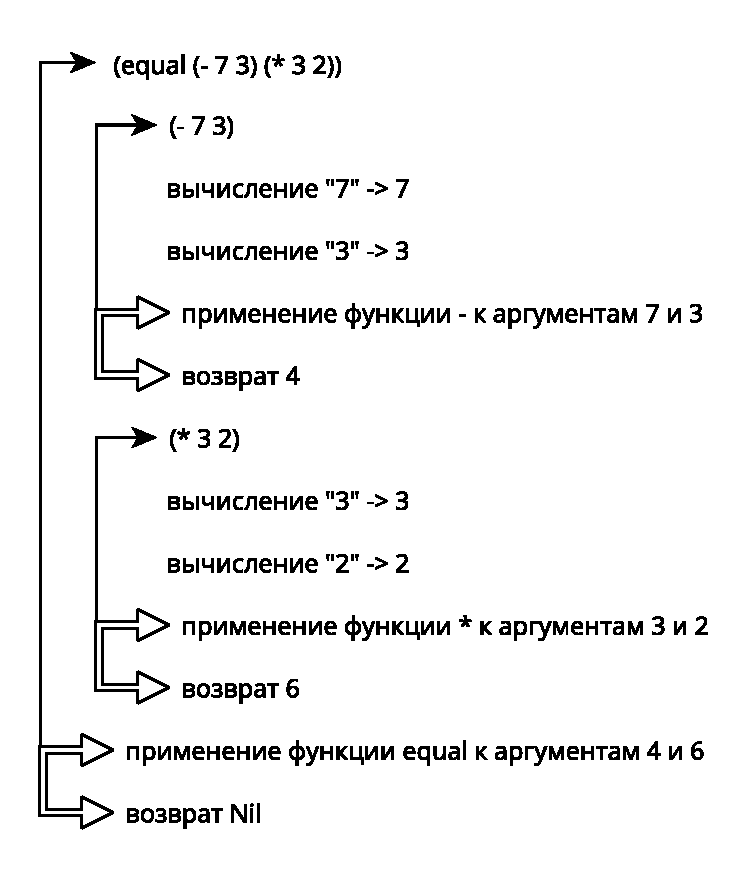
\includegraphics[width=0.5\linewidth]{1_5}
	\caption{Диаграмма вычисления выражения (equal (- 7 3) (* 3 2))}
	\label{1_5}
\end{figure}
\begin{figure}[H]
	\centering
	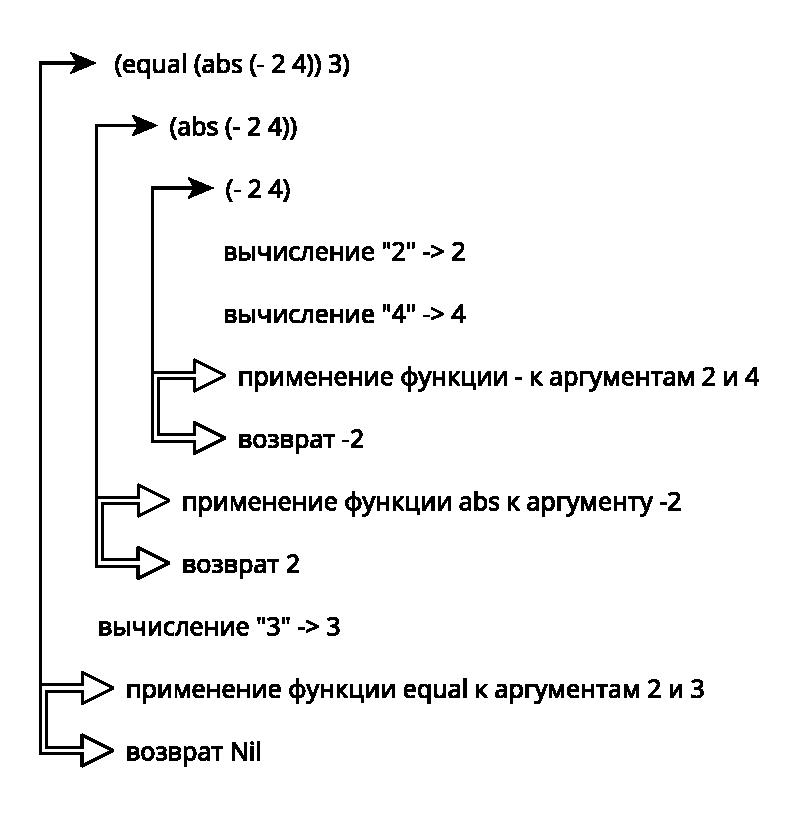
\includegraphics[width=0.5\linewidth]{1_6}
	\caption{Диаграмма вычисления выражения (equal (abs (- 2 4)) 3)}
	\label{1_6}
\end{figure}

\clearpage

\section{Задание 2. Написать функцию, вычисляющую гипотенузу прямоугольного треугольника по заданным катетам и составить диаграмму её вычисления}

\begin{lstlisting}
(defun hyp (a b)
	(sqrt 
		(+  ( * a a)
				( * b b))))
\end{lstlisting}
\begin{figure}[H]
	\centering
	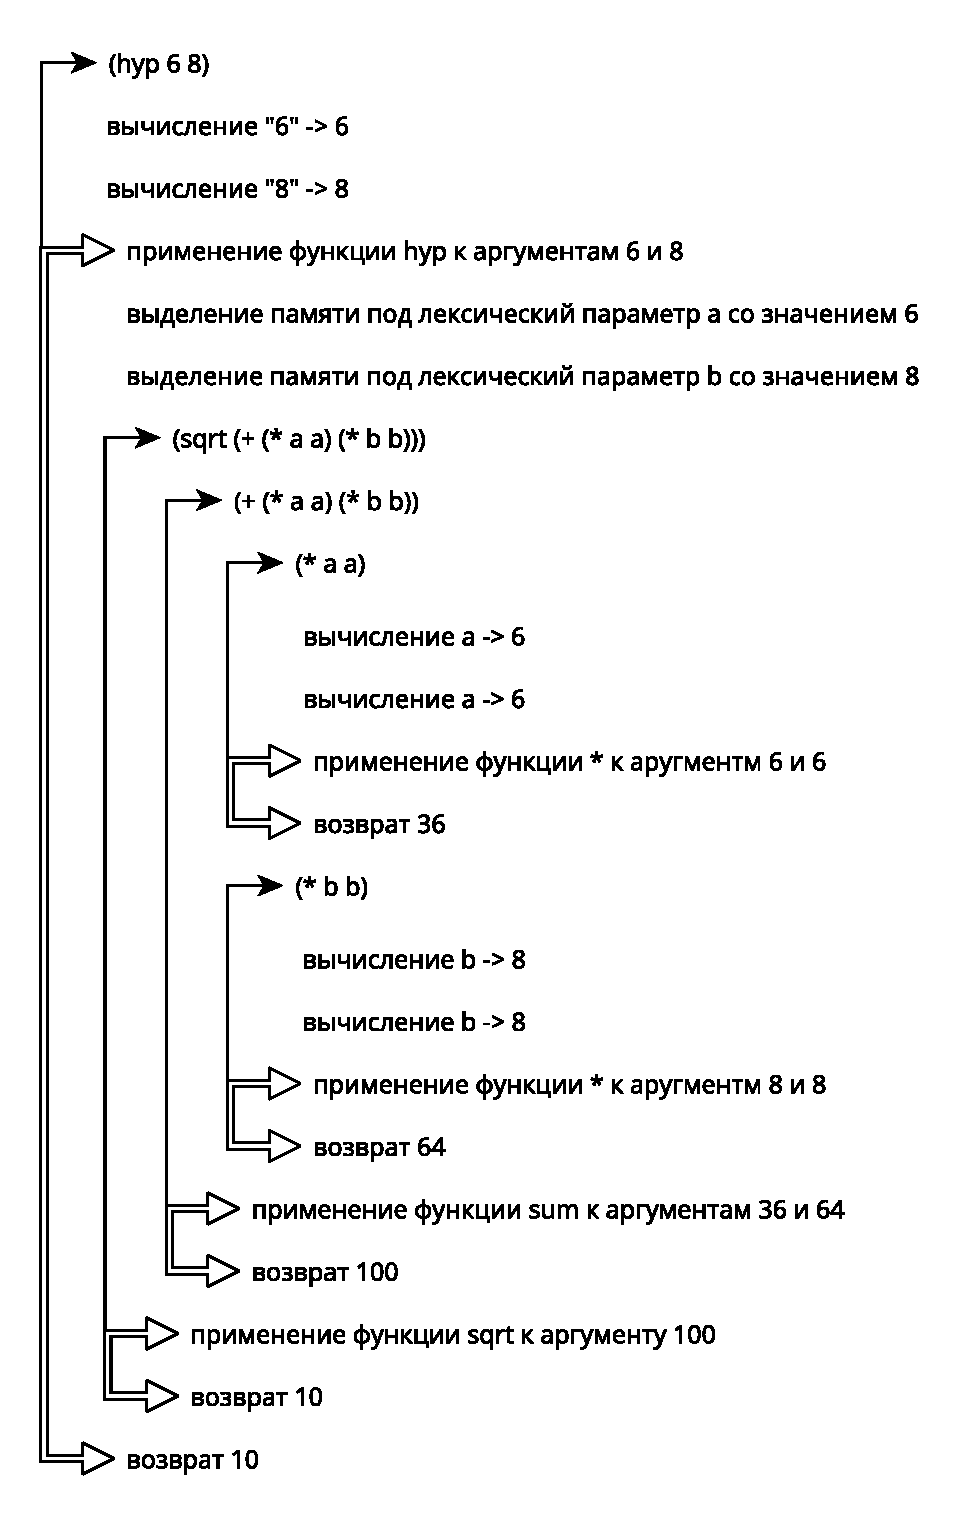
\includegraphics[width=0.6\linewidth]{2}
	\caption{Диаграмма вычисления выражения (hyp 6 8)}
	\label{2}
\end{figure}

\section{Задание 3. Каковы результаты вычисления следующих выражений?}

\begin{center}
	\begin{threeparttable}
		\captionsetup{justification=raggedright,singlelinecheck=off}
		\caption{\label{3}Результаты вычисления выражений}
		\centering
		\begin{tabular}{|c|c|c|}
			\hline
			Выражение & Результат & Исправление\\
			\hline
			(list 'a c) & variable C has no value & (list 'a 'c)\\
			\hline
			(cons 'a (b c)) & undefined function B & (cons 'a '(b c))\\
			\hline
			(cons 'a '(b c)) & (a b c) & ---\\
			\hline
			(caddr (1 2 3 4 5)) & 1 is not a function name & (caddr '(1 2 3 4 5))\\
			\hline
			(cons 'a 'b 'c) & too many arguments given to CONS & (cons 'a '(b c))\\
			\hline
			(list 'a (b c)) & undefined function B & (list 'a '(b c))\\
			\hline
			(list a '(b c)) & variable A has no value & (list 'a '(b c))\\
			\hline
			(list (+ 1 '(length '(1 2 3)))) & (length '(1 2 3)) is not a number & (list (+ 1 (length '(1 2 3))))\\
			\hline
		\end{tabular}
	\end{threeparttable}
\end{center}

\section{Задание 4. Написать функцию longer\_then от двух списков-аргументов, которая возвращает Т, если первый аргумент имеет большую длину}

\begin{lstlisting}
(defun longer_then (list1 list2)
	(>  (length list1)
			(length list2)))
\end{lstlisting}

\section{Задание 5. Каковы результаты вычисления следующих выражений?}

\begin{center}
	\captionsetup{justification=raggedright,singlelinecheck=off}
	\begin{longtable}[c]{|c|c|}
		\caption{\label{5}Результаты вычисления выражений}\\
		\hline
		Выражение & Результат \\
		\hline
		(cons 3 (list 5 6)) & (3 5 6)\\
		\hline
		(list 3 'from 9 'lives (- 9 3)) & (3 from 9 lives 6)\\
		\hline
		(+ (length for 2 too)) (car '(21 22 23))) & variable FOR has no value\\
		\hline
		(cdr '(cons is short for ans)) & (is short for ans)\\
		\hline
		(car (list one two)) & variable ONE has no value\\
		\hline
		(cons 3 '(list 5 6)) & (3 list 5 6)\\
		\hline
		(car (list 'one 'two)) & one\\
		\hline
	\end{longtable}
\end{center}

\section{Задание 6. Дана функция\\(defun mystery (x) (list (second x) (first x))). Какие результаты вычисления следующих выражений?}

\begin{center}
	\begin{threeparttable}
		\captionsetup{justification=raggedright,singlelinecheck=off}
		\caption{\label{6}Результаты вычисления выражений}
		\centering
		\begin{tabular}{|c|c|}
			\hline
			Выражение & Результат\\
			\hline
			(mystery (one two)) & undefined function ONE\\
			\hline
			(mystery (last one two)) & variable ONE has no value\\
			\hline
			(mystery free) & variable FREE has no value\\
			\hline
			(mystery one 'two)) & variable ONE has no value\\
			\hline
		\end{tabular}
	\end{threeparttable}
\end{center}

\section{Задание 7. Написать функцию, которая переводит температуру в системе Фаренгейта температуру по Цельсию (defum f-to-c (temp)…). Как бы назывался роман Р.Брэдбери <<451 по Фаренгейту>> в системе по Цельсию?}

\begin{lstlisting}
(defun f-to-c (temp)
	( * (/ 5 9)
			(- temp 32.0)))
\end{lstlisting}

Роман <<451 по Фаренгейту>> назывался бы <<232.77779 по Цельсию>>.

\section{Что получится при вычисления каждого из выражений?}

\begin{center}
	\begin{threeparttable}
		\captionsetup{justification=raggedright,singlelinecheck=off}
		\caption{\label{8}Результаты вычисления выражений}
		\centering
		\begin{tabular}{|c|c|}
			\hline
			Выражение & Результат\\
			\hline
			(list 'cons t NIL) & (cons t NIL)\\
			\hline
			(eval (eval (list 'cons t NIL))) & undefined function T\\
			\hline
			(apply $\sharp$cons ''(t NIL)) & bad syntax for complex number: $\sharp$CONS\\
			\hline
			(list 'eval NIL) & (eval NIL)\\
			\hline
			(eval (list 'cons t NIL)) & (t)\\
			\hline
			(eval NIL) & NIL\\
			\hline
			(eval (list 'eval NIL)) & NIL\\
			\hline
		\end{tabular}
	\end{threeparttable}
\end{center}

\clearpage